\let\negmedspace\undefined
\let\negthickspace\undefined
\documentclass[journal]{IEEEtran}
\usepackage[a5paper, margin=10mm, onecolumn]{geometry}
%\usepackage{lmodern} % Ensure lmodern is loaded for pdflatex
\usepackage{tfrupee} % Include tfrupee package

\setlength{\headheight}{1cm} % Set the height of the header box
\setlength{\headsep}{0mm}     % Set the distance between the header box and the top of the text

\usepackage{gvv-book}
\usepackage{gvv}
\usepackage{cite}
\usepackage{amsmath,amssymb,amsfonts,amsthm}
\usepackage{algorithmic}
\usepackage{graphicx}
\usepackage{textcomp}
\usepackage{xcolor}
\usepackage{txfonts}
\usepackage{listings}
\usepackage{enumitem}
\usepackage{mathtools}
\usepackage{gensymb}
\usepackage{comment}
\usepackage[breaklinks=true]{hyperref}
\usepackage{tkz-euclide} 
\usepackage{listings}
% \usepackage{gvv}                                        
\def\inputGnumericTable{}                                 
\usepackage[latin1]{inputenc}                                
\usepackage{color}                                            
\usepackage{array}                                            
\usepackage{longtable}                                       
\usepackage{calc}                                             
\usepackage{multirow}                                         
\usepackage{hhline}                                           
\usepackage{ifthen}                                           
\usepackage{lscape}
\usepackage{circuitikz}
\usepackage{tikz}
\usepackage{amsmath}
\usepackage{array}
\usepackage{tikz}
\usetikzlibrary{positioning}



\begin{document}

\bibliographystyle{IEEEtran}
\vspace{3cm}
\title{2022-GATE-ME-53-65}
\author{EE24BTECH11028 - Jadhav Rajesh}
% \maketitle
% \newpage
% \bigskip
{\let\newpage\relax\maketitle}

\renewcommand{\thefigure}{\theenumi}
\renewcommand{\thetable}{\theenumi}
\setlength{\intextsep}{10pt} % Space between text and floats


\numberwithin{equation}{enumi}
\numberwithin{figure}{enumi}
\renewcommand{\thetable}{\theenumi}

 \begin{enumerate}
     \item A schematic of an epicyclic gear train is shown in the figure. The sun $\brak{gear 1}$ and planet $\brak{gear 2}$ are external, and the ring gear $\brak{gear 3}$ is internal. Gear $1$, gear $3$ and arm $OP$ are pivoted to the ground at $O$. Gear $2$ is carried on the arm $O$P via the pivot joint at $P$, and is in mesh with the other two gears. Gear $2$ has $20$ teeth and gear $3$ has $80$ teeth. If gear $1$ is kept fixed at $0$ rpm and gear $3$ rotates at $900$ rpm counter clockwise $\brak{ccw}$, the magnitude of angular velocity of arm $OP$ is   $\_\_\_\_$ rpm $\brak{in integer}$.
     
\begin{figure}[h!]
         \centering
        
\includegraphics[width=0.7\linewidth]{figure/fig1/fig1.pdf}
		\caption{}
        \label{stemplot}

\end{figure}

     \item Under orthogonal cutting condition, a turning operation is carried out on a metallic workpiece at a cutting speed of $4 m/s$. The orthogonal rake angle of the  cutting tool is $5\degree$. The uncut chip thickness and width of cut are $0.2 mm$ and $3 mm$,respectively. In this turning operation ,the resulting friction angle and shear angle are $45\degree$ and $25\degree$, respectively. If the dynamic yield shear strength of the workpiece material under this cutting condition is $1000 MPa$, then the cutting force is $\_\_\_\_N\brak{round off to one decimal place}$.\\
     \item A $1 mm$ thick cylindrical tube, $100 mm$ in diameter, is orthogonally turned such that the entire wall thickness of the tube is cut in a single pass. The axial feed of the tool is $1 m/minute$ and the specific cutting energy $\brak{u}$ of the tube material is $6 j/mm^{3}$.Neglect contribution of feed force towards power.  The power required to carry out this operation $\_\_\_\_ kW \brak{round off to one decimal place}$.\\
     \item A $4 mm$ thick aluminum sheet of width $w=100 mm$ is rolled in a two-roll mill of roll diameter $200 mm$ each. The workpiece is lubrication with a mineral oil, which given a coefficient of friction, $\mu=0.1$. The flow stress $\brak{\sigma}$ of the material in MPa is $\sigma=207+ 414 \xi$, where $\xi$ is the true strain. Assuming rolling to be a plane strain deformation process, the roll separation force $\brak{F}$ for maximum permissible draft $\brak{thickness reduction}$ is $\_\_\_\_kN \brak{round off to nearest integer}$.\\
     Use:\\
     $F = 1.15 \Bar{\sigma} \brak{1+\frac{\mu L}{2h}}$WL,where $\bar{\sigma}$ is average flow stress, $L$ is roll-workpiece contact length, and $\bar{h}$ is the average sheet thickness.\\
     \item Two mild steel plates of similar thickness, in butt-joint configuration, are welded by gas tungsten arc welding process using the following welding parameters.\\
\begin{table}[h!]
\centering
\renewcommand{\arraystretch}{1.5}
\begin{tabular}{|m{5cm}|m{3cm}|}
    \hline
    \textbf{Welding voltage} & \textbf{20 V} \\ 
    \hline
    \textbf{Welding current} & \textbf{150 A} \\ 
    \hline
    \textbf{Welding speed} & \textbf{5 mm/s} \\ 
    \hline
\end{tabular}
\end{table}\\
     A filler wire of the same mild steel material having $3 mm$ diameter is used in this welding process. The filler wire feed rate is selected such that the final weld bead is composed of $60\%$ volume of filler and $40\%$ volume of plate material. The heat transfer factor is $0.7$ and melting factor is $0.6$. The feed rate of the filler wire is $\_\_\_\_ mm/s \brak{round off to one decimal place}$.\\
     \item An assignment problem is solved to minimize the total processing time of four jobs $\brak{1,2,3 and 4}$ on four different machines such that each job is processed exactly by one machine and each machine processes exactly one job. The minimum total processing time is found to be $500$ minutes. Due to a change in design, the processing time of job $4$ on each machine has increased by $20$ minutes. The revised minimum total process time will be $\_\_\_\_$ minutes $\brak{in integer}$.\\
     \item The product structure diagram shows the number of different components required 
     at each level to produce one unit of the final product $P$. If there are $50$ units of on-hand inventory of component $A$, the number of additional units of component $A$ needed to produce $10$ units of product $10$ units of $P$ is $\_\_\_\_ \brak{in integer}$.\\
\begin{tikzpicture}[
  level distance=1.5cm,
  level 1/.style={sibling distance=4cm},
  level 2/.style={sibling distance=3cm},
  level 3/.style={sibling distance=2cm},
  every node/.style={draw, rectangle, minimum width=1.5cm, minimum height=1cm}
  ]

% Root node
\node {P (1)}
  % Level 1 nodes
  child {node {A (4)}}
  child {node {B (2)}
    % Level 2 nodes
    child {node {C (1)}}
    child {node {D (3)}
      % Level 3 node
      child {node {A (2)}}
    }
  };
\end{tikzpicture}
     \item Consider a one-dimensional steady heat conduction process through a solid slab of 
     thickness $0.1 m$. The higher temperature side $A$ has a surface temperature of $80\degree^{c}$, and the heat transfer rate per unit area to low temperature side $B$ is$ 4.5 kW/m^{2}$. The thermal conductivity of the slab is $15 W/m.K$. The rate of entropy generation per unit area during the heat transfer process is $\_\_\_\_ W/m^{2}.K \brak{round off to 2 decimal places}$.\\
     \item In a steam power plant based on Rankine cycle, steam is initially expanded in a 
     high-pressure turbine. The steam is then reheated in a reheater and finally expanded in a low-pressure turbine. The expansion work in the high-pressure turbine is $400 kJ/kg$ and in the low-pressure turbine is $850 kJ/kg$, whereas the pump work is $15 kJ/kg$. If the cycle effiecient is $32\%$, the heat rejected in the condenser is $\_\_\_\_kJ/kg \brak{round off to 2 decimal places}$.\\
     \item An engine running on an air standard Otto cycle has a displacement volume $250 cm^{3}$
     and a clearance volume $35.7 cm^{3}$. The pressure and temperature at the beginning of the compression process are $100 kPa$ and $300 K$, respectively. Heat transfer during constant-volume heat addition process is $800 kJ/kg$. The specific heat at constant volume is $0.718 kJ/kg.K$ and the ratio of specific heats at constant pressure and constant volume is $1.4$. Assume the specific heats to remain constant during the cycle. The maximum pressure in the cycle is$\_\_\_\_ kPa \brak{round off to the nearest integer}$.\\
     \item A steady two-dimensional flow field is specified by the stream function\\
                      $\psi=kx^{3}y$,\\
     where $x$ and $y$ are in meter and the constant $k=1 m^{-2}s^{-1}$. The magnitude of acceleration at a point $\brak{x,y}=\brak{1 m,1 m}$ is $\_\_\_\_m/s^{2} \brak{round off to 2 decimal places}$.\\
     \item Consider a solid slab $\brak{thermal conductivity, k=10 W^{-1}K^{-1}}$ with thickness $0.2 m$ and of infinite extent in the other two direction as shown in the figure.Surface $2$, at $300 k$, is exposed to a fluid flow at a free stream temperature $\brak{T\infty}$ of $293 K$,with a convectivee heat transfer coefficient $\brak{h}$ of $00 Wm^{1}K^{1}$. Surface $2$ is opaque, diffuse and gray with an emissivity $\brak{\xi}$ of $0.5$ and exchanges heat by radiation with very ladge surroundings at $0 K$. Radiative heat transfer inside the solid slab is neglected. The stefan-Boltzmann constant is $5.67*10^{-8}Wm^{_2}K^{-4}$. The temperature $T_{1}$ of surface $1$ of the slab, under steady-state conditions, is $\_\_\_\_K \brak{round off to the integer}$.\\
\begin{figure}[h!]
         \centering
        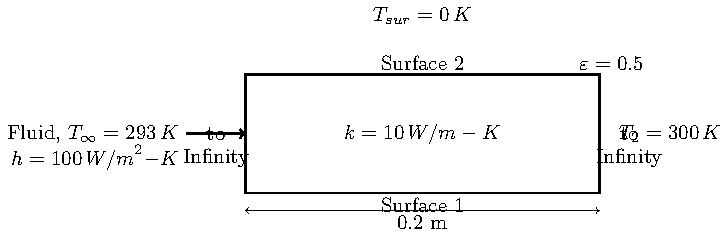
\includegraphics[width=0.7\linewidth]{figure/fig2/fig2.pdf}
		\caption{}
        \label{stemplot}

\end{figure}

     \item During open-heart surgery,a patient's blood is cooled down to $25\degree C$ from $37\degree C$ using a concentric tube counter-flow heat exchanger. Water enters the surgey is $5 L/minute$.\\
     Use the folowing fluid properties:\\
\begin{table}[h!]
\centering
\begin{tabular}{|c|c|c|}
\hline
\textbf{Fluid} & \textbf{Density (kg/m$^3$)} & \textbf{Specific heat (J/kg-K)} \\
\hline
Blood & 1050 & 3740 \\
\hline
Water & 1000 & 4200 \\
\hline
\end{tabular}
\caption{Properties of fluids}
\end{table}\\
     Effectiveness of the heat exchanger is $\_\_\_\_ \brak{round off to 2 decimal places}$.





     
 \end{enumerate}



\end{document}
